\documentclass[10pt]{article}
\usepackage{ctex}
\usepackage{graphicx}
\graphicspath{{E:/大学课程/大一下/人工智能程序设计/作业集/第二次作业/},{pics/}}
\usepackage{amsmath}
\usepackage{amssymb}
\usepackage{float}%使图片紧跟在文字后面


\title{第二周平时作业}
\author{朱士杭\ 231300027}
\date{\kaishu \today}


\begin{document}
	\maketitle
\section{问题一}
	\subsection{直接赋值}
	将变量名指向对象,对象及其id不变,变的只是变量的指向\par
	比如:x=3,y=3,y=4  一开始x和y都指向对象3,后来y改变指向指向对象4\par
	又比如:list1=[1,2,[3,3]]  list2=list1  此时list1和list2的id都是一样的,指向的对象是一样的,对list1的改变相当于在对list2进行改变
	\subsection{Copy方法}
	将对象整体复制一份新的,但是对象内部的元素对象id不会发生改变\par
	比如:list1=[1,2,[3,3]]  list2=list1.copy()  此时list1和list2的id不一样,但是for循环输出之后会发现list1和list2里面的对象的id是一样的,这就意味着改变list1里的1或2没关系,但一旦改变[3,3]对象里的元素时,list2里面的[3,3]也会跟着发生改变,这就牵扯到接下来需要说的有关于深拷贝deepcopy的问题
	\subsection{Deepcopy方法}
	from copy import deepcopy\par
	通过深拷贝将list1和list2里面的对象都赋予其新的id,对其中一个的改变不会影响另一个

\section{问题二}	
	\subsection{mutable可变对象}
	id是会随着操作发生改变的对象,比如说列表、字典、集合\par
	比如:list1=[1,2,3]其id为140728001318144  进行改变操作之后list1[1]=10其id变为1914524434752
	\subsection{immutable不可变对象}
	id一旦形成就是确定好的没有办法发生改变的对象\par
	比如说整数、浮点数、元组、字符串

\section{问题三}	
	\subsection{程序一}
	会输出:[['\_','\_','\_'],['\_','\_','X'],['\_','\_','\_']]\par
	原因:通过列表解析,每一次创建的列表都是指向一个新的对象['\_','\_','\_']对其中一个['\_','\_','\_']列表的改变不会影响其他列表
	\subsection{程序二}
	会输出:[['\_','\_','X'],['\_','\_','X'],['\_','\_','X']]\par
	直接通过[]*3列表乘3的操作来实现二维列表的拼接,本质上是复制了3份指向同一个['\_','\_','\_']对象的变量名,对其中一个的改变相当于在对另外两个列表进行相同的改变
\section{问题四}
		\subsection{Packing}
		打包操作,使用可迭代解包运算符在单个变量中收集多个值,个人理解就是在迭代一个对象的时候从里面将多个值囊括进一个新的对象\par
		比如:a,*b,c=[1,2,3,4]\quad 其中b就是[2,3]这里就是一个packing
		\subsection{Unpacking}
		解包操作,在单个赋值语句中将可迭代的值分配给变量的元组(或列表)\par
		比如一个基本的赋值语句就是a,b=1,2,将元组(1,2)进行解包之后分别分配给对象(a,b)中的元素
		\subsection{综合Packing与Unpacking}
			\begin{figure}[H]
			\centering
			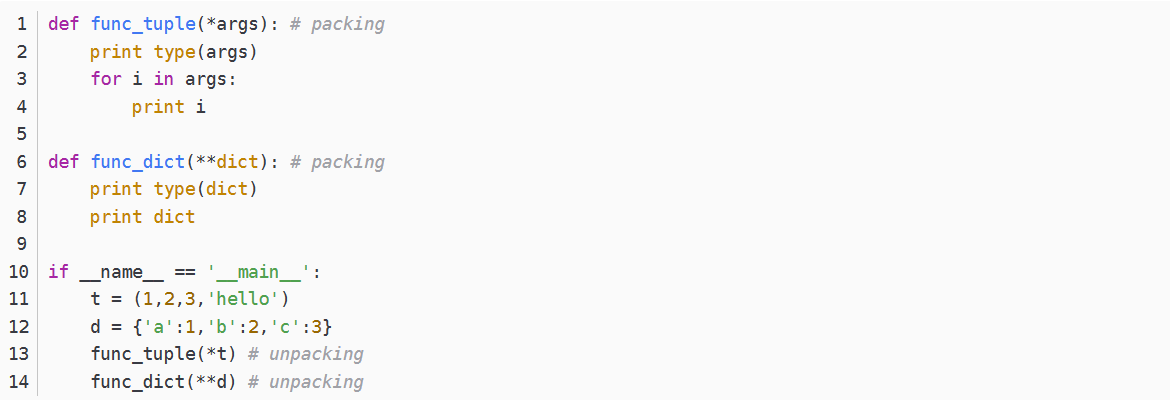
\includegraphics[scale=0.6]{Packing和Unpacking}
			\caption{Packing和Unpacking}
			\end{figure}
		\subsection{*args及其作用}
		*args是一个特殊的语法,用于在函数定义中收集任意数量的位置参数。这里的args是参数名,可以是任何合法的变量名,通常约定使用args,但也可以是其他名称。星号*表示将接收的所有位置参数打包成一个元组tuple,这样在函数中可以遍历它来处理所有的参数
		\subsection{参考资料}
		ps.第四问一开始不知道答案通过查找相关资料才得出结果,参考链接如下:\par
		https://blog.csdn.net/linux4fun/article/details/16803937\par
		https://blog.csdn.net/qq\_27825451/article/details/81666601\par
		https://zhuanlan.zhihu.com/p/639405308
\section{问题五——自行创建字典}
		\begin{figure}[H]
			\centering
			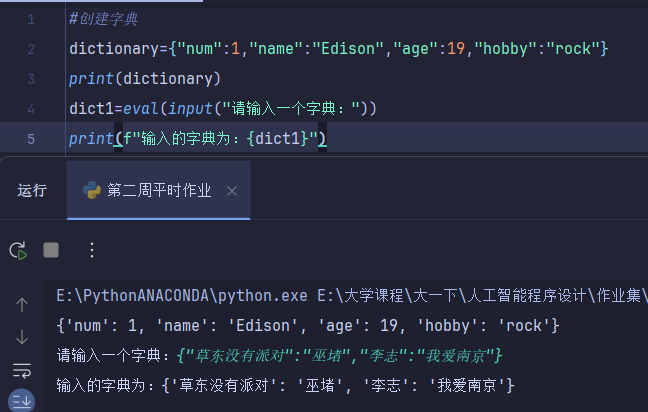
\includegraphics[scale=0.6]{创建简单字典}
			\caption{创建简单字典}
		\end{figure}
		\noindent{代码如下:}\\
		$dictionary=\left\{"num":1,"name":"Edison","age":19,"hobby":"rock" \right\} \\$
		print(dictionary)\\
		dict1=eval(input(``请输入一个字典:''))\\
	    print(f``输入的字典为:$\left\{dict1\right\}'')$
		
\end{document}

